%\documentclass[aps,prb,onecolumn,nofootinbib]{revtex4}  
\documentclass[12pt,a4paper]{article}
\usepackage[margin=1in]{geometry}  % set the margins to 1in on all sides
%\usepackage{jheppub}
\usepackage{amsmath,amsfonts,amssymb,latexsym}
\usepackage{hhline}
\usepackage{graphicx}
\usepackage[arrow,matrix]{xy}
\usepackage{tikz}
\usepackage{tikz-cd}
\usetikzlibrary{positioning,arrows}
\usetikzlibrary{decorations.pathmorphing}
\usetikzlibrary{decorations.markings}
\newcommand{\tp}{\otimes}
\newcommand{\ra}{\rightarrow}
\newcommand{\unit}{\mathbf{1}}
\newcommand{\zz}{\mathbb{Z}}
\newcommand{\mce}{\mathcal{E}}
\newcommand{\cc}{\mathbb{C}}
\newcommand{\rr}{\mathbb{R}}
\newcommand{\mcr}{\mathcal{R}}
\newcommand{\mcz}{\mathcal{Z}}
\newcommand{\mca}{\mathcal{A}}
\newcommand{\mcg}{\mathcal{G}}
\newcommand{\mct}{\mathcal{T}}
\newcommand{\ul}{\underline}
\newcommand{\Mod}{\text{Mod}}
\newcommand{\Aut}{\text{Aut}}
\newcommand{\ulmcc}{\underline{\mathcal{C}}}
\newcommand{\zt}{\mathbb{Z}_2}
\newcommand{\oeo}{\text{others = 1}}
\newcommand\be            {\begin{equation}}
\newcommand\ee            {\end{equation}}
\newcommand\ba            {\begin{aligned}}
\newcommand\ea            {\end{aligned}}
\newcommand{\mcf}{\mathcal{F}}
\newcommand{\spinz}{\text{\sffamily{Z}}}
\newcommand{\spinx}{\text{\sffamily{X}}}
\newcommand{\mcl}{\mathcal{L}}
\newcommand{\mcc}{\mathcal{C}}
\newcommand{\mco}{\mathcal{O}}
\newcommand{\mcm}{\mathcal{M}}
\newcommand{\zc}{\mathcal{Z}(\mathcal{C})}
\newcommand{\id}{\text{id}}
\newcommand{\Hom}{\text{Hom}}
\newcommand{\End}{\text{End}}
\newcommand{\Tor}{\text{Tor}}
\newcommand{\Ext}{\text{Ext}}
\newcommand{\p}{\partial}
\newcommand{\wt}{\widetilde}
\usepackage{verbatim}
\newcommand{\cl}{\mathbb{C}\ell}
\newcommand{\vect}{\text{Vec}}
\newcommand{\svect}{\text{sVec}}
\newtheorem{thm}{Theorem}
\newtheorem{cor}{Corollary}
\newtheorem{lemma}{Lemma}
\newtheorem{prop}{Proposition}
\newtheorem{problem}{Problem}
\newtheorem{defn}{Definition}
\newtheorem{question}{Question}
\newcommand{\fube}{\textbf{Fube}}
\newcommand{\fld}{\mathcal{F}}
\newcommand{\dave}[1]{{\color{red}\footnotesize{(DA) #1}}}

%a purple that looks different from red. EL: nice! I like the name
\definecolor{amethyst}{rgb}{0.6, 0.4, 0.8}
\newcommand{\ethan}[1]{{\color{amethyst}\footnotesize{(EL) #1}}}

\newcommand{\CapDotLeft}{\mathord{\vcenter{\hbox{
\includegraphics[scale=1]{CapDotLeft.pdf}}}}}
\newcommand{\CapDotRight}{\mathord{\vcenter{\hbox{
\includegraphics[scale=1]{CapDotRight.pdf}}}}}
\newcommand{\CupDotLeft}{\mathord{\vcenter{\hbox{
\includegraphics[scale=1,angle=180,origin=c]{CapDotRight.pdf}}}}}
\newcommand{\CupDotRight}{\mathord{\vcenter{\hbox{
\includegraphics[scale=1,angle=180,origin=c]{CapDotLeft.pdf}}}}}

\newcommand{\CupCap}{\mathord{\vcenter{\hbox{
\includegraphics[scale=1]{CupCap.pdf}}}}}
\newcommand{\CupCapDots}{\mathord{\vcenter{\hbox{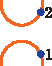
\includegraphics[scale=1]{CupCapDots.pdf}}}}}

\newcommand{\SigmaDotDot}{\mathord{\vcenter{\hbox{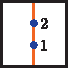
\includegraphics[scale=1]{SigmaDotDot.pdf}}}}}
\newcommand{\SigmaDotDotExchange}{\mathord{\vcenter{\hbox{
\includegraphics[scale=1]{SigmaDotDotExchange.pdf}}}}}
\newcommand{\TwoLine}{\mathord{\vcenter{\hbox{
\includegraphics[scale=1]{TwoLine.pdf}}}}}
\newcommand{\TwoLineDots}{\mathord{\vcenter{\hbox{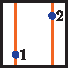
\includegraphics[scale=1]{TwoLineDots.pdf}}}}}

\newcommand{\RDotTwo}{\mathord{\vcenter{\hbox{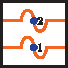
\includegraphics[scale=1]{RDotTwo.pdf}}}}}
\newcommand{\RDotTwoa}{\mathord{\vcenter{\hbox{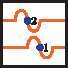
\includegraphics[scale=1]{RDotTwoa.pdf}}}}}
\newcommand{\RDotTwob}{\mathord{\vcenter{\hbox{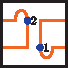
\includegraphics[scale=1]{RDotTwob.pdf}}}}}
\newcommand{\RDotTwoc}{\mathord{\vcenter{\hbox{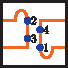
\includegraphics[scale=1]{RDotTwoc.pdf}}}}}

\newcommand{\FubeXXX}{\mathord{\vcenter{\hbox{
\includegraphics[scale=1]{EmptyTube.pdf}}}}}
\newcommand{\FubeXss}{\mathord{\vcenter{\hbox{
\includegraphics[scale=1]{OneLine.pdf}}}}}
\newcommand{\FubeXsds}{\mathord{\vcenter{\hbox{
\includegraphics[scale=1]{OneLineDot.pdf}}}}}

\newcommand{\FubesXs}{\mathord{\vcenter{\hbox{
\includegraphics[scale=1,angle=90,origin=c]{OneLine.pdf}}}}}
\newcommand{\FubesdXs}{\mathord{\vcenter{\hbox{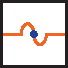
\includegraphics[scale=1]{FubesdXs.pdf}}}}}

\newcommand{\FubessX}{\mathord{\vcenter{\hbox{
\includegraphics[scale=1]{FubessX.pdf}}}}}
\newcommand{\FubessdX}{\mathord{\vcenter{\hbox{
\includegraphics[scale=1]{FubessdX.pdf}}}}}

\newcommand{\FubesXsa}{\mathord{\vcenter{\hbox{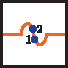
\includegraphics[scale=1]{FubesXsa.pdf}}}}}
\newcommand{\FubesXsb}{\mathord{\vcenter{\hbox{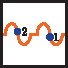
\includegraphics[scale=1]{FubesXsb.pdf}}}}}
\newcommand{\FubesXsc}{\mathord{\vcenter{\hbox{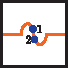
\includegraphics[scale=1]{FubesXsc.pdf}}}}}


\newcommand{\qqo}{\mathord{\vcenter{\hbox{\includegraphics[scale=.4]{qq1.pdf}}}}}
\newcommand{\qtqo}{\mathord{\vcenter{\hbox{\includegraphics[scale=.4]{qtq1.pdf}}}}}
\newcommand{\qqto}{\mathord{\vcenter{\hbox{\includegraphics[scale=.4]{qqt1.pdf}}}}}
\newcommand{\qtqto}{\mathord{\vcenter{\hbox{\includegraphics[scale=.4]{qtqt1.pdf}}}}}
\newcommand{\qqm}{\mathord{\vcenter{\hbox{\includegraphics[scale=.4]{qqm.pdf}}}}}
\newcommand{\qtqm}{\mathord{\vcenter{\hbox{\includegraphics[scale=.4]{qtqm.pdf}}}}}
\newcommand{\qqtm}{\mathord{\vcenter{\hbox{\includegraphics[scale=.4]{qqtm.pdf}}}}}
\newcommand{\qtqtm}{\mathord{\vcenter{\hbox{\includegraphics[scale=.4]{qtqtm.pdf}}}}}



\begin{document}


\title{First thoughts about fermions}

\author{Ethan Lake}
%\affiliation{Department of Physics and Astronomy, University of Utah, Salt Lake City, UT 84112, USA}
%\emailAdd{lake@physics.utah.edu}
\date{\today}

\maketitle

\tableofcontents

\section{Background material} 

\subsection{Supervector spaces and other superstuff}
 
In order to think about fermionic topological phases, it's helpful to go back and recall that objects in tensor 
categories can usually be interpreted in terms of vector spaces. Since we're working with unitary TQFTs we will be working over $\cc$ and come equipped with a natural tensor product $\tp_\cc$, and so the simple objects in our categories can be regarded as simple $\cc$-algebras. 

When our theories arise from fermionic degrees of freedom, we need to keep track of fermion parity. We can do this by splitting all vector spaces up into a direct sum of their fermion-parity even and fermion-parity odd sectors, writing $V = V^0 \oplus V^1$. This decomposition turns vector spaces into {\it supervector spaces}, which are just $\zt$-graded versions of regular vector spaces. Throughout we will use the operator $P$ as the fermion parity operator, defined by $Pv = v$ if $v\in V^0$ (even fermion parity) and $Pv = -v $ if $v\in V^1$ (odd fermion parity). 

The tensor product of two supervector spaces works in the obvious way:
\be (V\tp W)^0 = V^0 \tp W^0 \oplus V^1 \tp W^1,\quad (V\tp W)^1 = V^0 \tp W^1 \oplus V^1 \tp W^0.\ee
We will use absolute value bars to denote the parity of vectors in supervector spaces. That is, for $v\in V$, we write $|v| = 0$ if $Pv = v$ (i.e. if $v\in V^0$) and $|v| = 1$ if $Pv = -v$ (i.e. if $v\in V^1$). The tensor product between vectors in supervector spaces is supercommutative, in the sense that it supercommutes in the same way that differential forms supercommute:
\be v\tp w = (-1)^{|v||w|}w\tp v.\ee
This means that sVec (the category of supervector spaces) naturally comes equipped with the structure of a braided category. 

If a supervector space $V$ has $\dim V^0 = a$ and $\dim V^1 = b$, we say that $V$ has superdimension $a|b$. We will use the notation $\cc^{a|b}$ to denote the supervector space of superdimension $a|b$. To put it another way, $\cc^{a|b}$ is a $(a+b)$-dimensional vector space with $a$ fermion-parity even generators and $b$ fermion-parity odd generators. 

When we tensor $\cc^{a|b}$ with $\cc^{c|d}$, the graded dimensions behave in the same way that supervector spaces behave when you tensor them together. That is, they behave just like you would expect: 
\be  \cc^{a|b}\tp \cc^{c|d} \cong \cc^{ac + bd | ad + bc}.\ee
Notice in particular that $\cc^{a|b} \tp \cc^{1|0} \cong \cc^{a|b}$ and $\cc^{a|b} \tp \cc^{0|1} \cong \cc^{b|a}$. That is, tensoring with $\cc^{1|0} = \cc$ does nothing (as it should), and tensoring with $\cc^{0|1}$ is equivalent to flipping fermion parity. 

\subsection{Clifford algebras}

The supervector space $\cc^{1|1}$ will turn out to play an important role in what follows. This is because it is invariant under fermion-parity flips: $\cc^{1|1} \tp \cc^{0|1} \cong \cc^{1|1}$. It is also an example of a Clifford algebra, namely the Clifford algebra $\cl_1$. Clifford algebras will be important for us and show up whenever fermions are involved in anything, so we will quickly review their definition. 

The complex Clifford algebras $\cl_n$ are the supervector spaces generated by the number 1 and $n$ {\it parity-odd} generators $\gamma_1,\dots,\gamma_n$ which satisfy the relations 
\be \{\gamma_i,\gamma_j\} = 2Q_{ij},\ee
where $\{\gamma_i,\gamma_j\} = \gamma_i\tp \gamma_j + \gamma_j\tp\gamma_i$ and $Q_{ij}$ is some quadratic form, which for us can always be diagonalized. We will usually choose $Q_{ij} = \delta_{ij}$, although since we are working over $\cc$, this is equivalent to choosing a diagonal matrix with an arbitrary placement of $\pm1$s on the diagonal. 

The simplest (other than $\cl_0 = \cc$) Clifford algebra is $\cl_1 = \langle 1, \gamma\rangle$, with $\gamma^2 = 1$ and $P\gamma = -\gamma$. 
Since by definition $\cl_1$ has one even generator ($1$) and one odd generator ($\gamma$), we have $\cl_1 \cong \cc^{1|1}$. In terms of representations, we can choose a representation $\rho$ such that $\rho(1) = \unit_{2\times 2}$ and $\rho(\gamma) = \sigma^x$, which is consistent since $\{\sigma^x,\sigma^x\} = 2\unit_{2\times2}$ and $\sigma^x : \cc^{1|0} \mapsto \cc^{0|1}, \cc^{0|1}\mapsto \cc^{1|0}$, $i.e.$ $\sigma^x$ is odd. We will see that $\cl_1$ is the prototypical ``Majorana'' supervector space that will appear later on.

The whole structure of Clifford algebras is super interesting, although I'm not sure if we'll really need to refer to it in any detail in what follows. Just for posterity's sake though, we note that $\cl_n \cong \cl_1^{\tp n}$ and that $\cl_2 \cong \cl_1\tp \cl_1$ is actually $\cl_2 \cong \End(\cc^{1|1})$, which we might need later.% We can see this by choosing the representation $\rho(1) = \unit_{2\times2},\rho(\gamma_1)=\sigma^x,\rho(\gamma_2)=\sigma^y$. 

\subsection{Modules and Morita equivalence}\label{sec:morita}

A module over an algebra is a vector space whose scalars are drawn from the algebra. That is, it's a way of giving an algebra an action on a vector space. So modules are the algebra analogue of representations: representations construct a way for groups to act on vector spaces, and modules do the same thing for algebras. 

A mathematical concept that will be relevant is the notion of {\it Morita equivalence}. Roughly, Morita equivalence is a way of establishing when two algebras ``have the same modules'', or when their ``representation theory is the same''. The technical definition is that two algebras $A$ and $B$ are Morita equivalent (written $A\cong_M B$) when the cateogries of their left modules Mod$^L(A)$ and Mod$^L(B)$ are equivalent, although we won't use this definition much. 

The reason why the notion of Morita equivalence is useful for us is because quasiparticles in topological phases are identified with simple modules of an algebra $\fube$ called the {\it Fube algebra}, which we'll talk about in more detail later. Usually figuring out the algebra structure of \fube\ is straightforward, although computing its simple modules (aka finding an idepmpotent decomposition of \fube) can often be a huge pain. Since Morita equivalent algebras have the same modules, we can often replace a complicated fube algebra or a sub-algebra of a fube algebra with a much simpler but Morita equivalent algebra, which can greatly facilitate the determination of its simple modules.

The canonical example of Morita equivalent algebras are the matrix algebras. It turns out that we actually have $\cc(n) \cong_M \cc$ for all $n$ (where $\cc(n)$ are complex $n\times n$ matrices). This can be seen by using the following proposition:

\begin{prop}
Let $A,B$ be two algebras, and $\mce$ be an $A-B$ bimodule, that is, let $\mce$ be a left $A$-module and a right $B$-module. Suppose $\mce$ is such that 
\be \mce^* \tp_A \mce \cong B,\qquad \mce\tp_B \mce^* \cong A.\ee
Then $A$ and $B$ are Morita equivalent.
\end{prop}
We will do the proof by setting up the equivalence between the modules of $A$ and $B$ explicitly. Suppose $M$ is a module over $A$, and $N$ a module over $B$. Construct the functors $F : \Mod(A) \ra \Mod(B)$, $G:\Mod(B) \ra \Mod(A)$ as
\be F: M \mapsto \Hom_A(\mce,M),\qquad G : N \mapsto \mce\tp_B N.\ee
This associates $M$ with a $B$-module and $N$ with an $A$-module. We claim that this is an isomorphism, namely that $F$ and $G$ are inverses of one another. If this is true, we must have 
\be M \cong \mce\tp_B \Hom_A(\mce,M) \cong (\mce \tp_B \mce^*)\tp_A M,\qquad N\cong \Hom_A(\mce,\mce\tp_B N)\cong (\mce^*\tp_A\mce)\tp_BN,\ee
but this holds precisely due to our assumptions on $\mce\ \square$. 

The Morita equivalence between $\cc(n)$ and $\cc$ then follows from setting the bimodule $\mce$ to be $\mce = \cc^n$ in the above construction. 

As a useful nonexample, $\cc^n \not\cong_M \cc^m$ for any $n\neq m$. This can be seen by realizing that the centers of two Morita equivalent algebras must always be the same. This is true for the $\cc(n) \cong_M \cc$ example considered above, but of course the centers of $\cc^n$ and $\cc^m$ are different if $n\neq m$, and so indeed $\cc^n \not\cong_M \cc^m$. 

One useful fact that we will exploit in calculations is that two algebras $A$ and $B$ are always Morita equivalent if there exists a supervector space $V$ such that 
\be A \cong B \tp_\cc \End(V).\ee

For a useful example of this, we turn to the Clifford algebras. We will use the fact that  \be\cl_2 \cong \End(\cl_1) \cong \End(\cc^{1|1}),\ee
which can be seen just by realizing that $\End(\cl_1) \cong \cl_1 \tp \cl_1 \cong \cl_2$. This means that 
\be \cl_{n+2} \cong_M \cl_n\ee
for all $n$, and so $\cl_{n+2}$ and $\cl_n$ always have the same modules (this is Bott periodicity!). In particular, we see that $\cl_2$ has the same modules as $\cc$! This will be very helpful later on when we look at condensing fermions in the Ising theory. There, we will run into subalgebras of \fube\ that are isomorphic to $\End(\cc^{1|1})$. By what we've just seen these subalgebras must have the same modules as $\cc$, which is much easier to work with than $\cl_2$. Since the modules of the \fube\ algebra (and its subalgebras) determine the quasiparticles in the theory, which see in particular that subalgebras of \fube\ given by $\End(\cc^{1|1})$ must give rise to only a single quasiparticle, since we are free to replace them by the trivial algebra $\cc$. 


\section{Superfusion categories} 


When make go from fusion categories to superfusion categories, the simple objects become supervector spaces. This is the ``grading the vertices'' picture. Thus, understanding what happens to the objects is straightforward. 

However, the morphisms also become superspaces, which for us is very important. In particular, this means that all the Hom spaces ($a.k.a$ fusion spaces) carry a $\zt$-grading that keeps track of their fermion parity. In particular, $\Hom_\mcc(X,Y)^0$ contains all the morphisms between $X$ and $Y$ that leave the fermion parity of $X$ unchanged, and $\Hom_\mcc(X,Y)^1$ contains all the morphisms that reverse the fermion parity of $X$. For any morphism $f : X\ra Y$, we will write $|f| = 
0$ if $f$ is even (preserves fermion parity) and $|f| = 1$ if $f$ is odd (reverses fermion parity). 

Without loss of generality, we can consider fusion diagrams built from a tensor product of fusion spaces $\Hom_\mcc(X\tp Y,Z)$. Forming a fusion graph requires choosing basis vectors for all these fusion spaces. Following convention, we will write $s^{XY}_Z(\alpha)$ to denote the parity of the basis vector for the fusion space $\Hom_\mcc(X\tp Y,Z)$, where $1\leq\alpha\leq N^{XY}_Z$. For notational simplicity we will assume $N^{XY}_Z \leq 1$, so that all the fusion spaces are one-dimensional and have a unique fermion parity. Relaxing this constraint is of course straightforward, and just involves writing more indices. 

The grading of morphisms is important to keep track of, since morphisms satisfy their own supercommutativity law, called the {\it superexchange law}, which states that for any four morphisms $f,g,h,k \in \mcc$, we have
\be (f\tp g) \circ (h\tp k) = (-1)^{|g||h|}(f\circ g)\tp(g\circ k).\ee
This looks reasonable, but if you actually try to draw what this means, it looks a little odd. Futhermore, it's not really motivated in the literature anywhere, so let's run through how to see this. First of all, recall that in normal fusion categories, the tensor product of two morphisms is the same as horizontal superposition:
\be \includegraphics{ftpg.pdf}\ee
In {\it superfusion} categories, we need to be more careful, since morphisms (like $\Hom(X\tp Y,Z)$!) can carry nontrivial fermion parity. This is actually really easy to fix diagrammatically: we just write the tensor product of two morphisms in a displaced way, where the first morphism in the tensor product is displaced above the second:
\be \includegraphics{superftpg.pdf} \ee
Moving two morphisms past each other vertically may then result in a minus sign, since if both morphisms have odd fermion parity, moving them past each other is like exchanging two fermions. That is, 
\be \includegraphics{morphism_commutativity.pdf}\ee
With this crucial property, it's easy to verify the superexchange law (remember that composition of morphisms is the same as stacking of diagrams).



%The most important morphisms we'll be grading are the fusion spaces present in fusion diagrams. Since we assume that all the nonzero fusion spaces to be one-dimensional, we can let $H^{XY}_Z$ denote the basis vector of the space $\Hom(X\tp Y,Z)$, so that $|H^{XY}_Z| = s^{XY}_Z$. 


Finally, let's quickly mention the $F$-moves (we'll come back to them in more detail later). Recall that we can write them as the basis changes
\be [F^{ijk}_l] : \bigoplus_m \Hom(i\tp j,m) \tp \Hom(m\tp k,l) \cong \bigoplus_n \Hom(i\tp n,l) \tp \Hom(j\tp k,n).\ee
The $F$-moves shouldn't change the fermion parity of the fusion graph, and so the must be {\it even} morphisms. This means that the fermion parity on both sides of the above isomorphism must be the same. To quantify this condition, let $s^{ij}_m$ be the parity of the Hom space $\Hom(i\tp j,m)$. The even-ness of $F$ means that 
\be \label{scond}  s^{ij}_m + s^{mk}_l = s^{jk}_n + s^{in}_l.\ee
In particular, if $\mcc = \vect_G$ for some finite Abelian $G$, this is equivalent to the 2-cocycle condition, and so we see in particular that such theories are parametrized by a choice of cohomology class $s \in H^2(G,\zt)$. 

\subsection{Categorical caveats}\label{sec:ccs}
A number of formulae that we're used to using when working with fusion categories fail to hold upon passing to superfusion categories, while others go through unchanged. 
First, direct sums in superfusion categories factor out of $\Hom$s in the usual way:
\be \Hom(\bigoplus_i X_i,Y) \cong \bigoplus_i\Hom(X_i,Y),\qquad \Hom(X,\bigoplus_i Y_i) \cong \bigoplus_i\Hom(X,Y_i) .\ee
This happens in any (graded or otherwise) fusion category that we can cook up (at least provided we work with finitely many objects). 

However, consider the usual ``coproduct'' isomorphism which we're familiar with from regular category theory:
\be\label{copiso} \Hom(X,Y) \cong \bigoplus_{Z\in \mcc} \Hom(X,Z) \tp \Hom(Z,Y).\ee
This amounts to stitching $X$ and $Y$ together by summing over all the objects that can connect $X$ to $Y$. To put it in other words, consider the diagram
\be
\begin{tikzcd}
X \arrow[r] \arrow[dr, dashrightarrow]
& Z \arrow[d]\\
& Y
\end{tikzcd}
\ee
The isomorphism \eqref{copiso} says that going along the dashed arrow is equivalent to the sum of all the different ways to go along the two-arrow path. As physicists, we usually see \eqref{copiso} written as the resolution of the identity 
\be \Hom(X\tp Y,X\tp Y) \cong \bigoplus_{Z\in \mcc} \Hom(X\tp Y,Z) \tp \Hom(Z,X\tp Y),\ee
which diagrammatically looks like
\be \includegraphics{resid.pdf} \ee


These isomorphisms do {\it not} hold in general categories! The RHS of \eqref{copiso} will in general be much bigger than the left: the space of all maps through the top path of the diagram above will generically be much larger than the space of all maps along the dahsed arrow. 

The reason that \eqref{copiso} doesn't hold is due to nontrivial options for the endomorphism rings of simple objects that appear for superfusion categores. In the superfusion case, the big direct sum on the RHS of \eqref{copiso} needs to be replaced with a colimit, although since we aren't mathematicians we probably don't want to get too involved with colimits. %Also note that as a corollary of this, $\End(X) \tp \End(Y)\not\cong\End(X\tp Y)$ in general.

There's actually a simple way to fix \eqref{copiso} without thinking about colimits, and it involves changing the type of tensor product we use. We've tacitly been assuming that all of our tensor products are secretly $\tp_\cc$, tensor products over $\cc$. This works only because in regular categories the Hilbert spaces associated with worldlines are always $\cc$. However, we run into problems if we have objects with $\End(Z) \not\cong \cc$ and continue to use $\tp_\cc$. If $\End(Z)$ is bigger than $\cc$, then the RHS of \eqref{copiso} is bigger than the LHS, since the internal $Z$ leg of the fusion diagram contributes a larger space to the direct sum. This is unphysical though, since the internal worldlines of freedom $Z$ shouldn't carry any more information than is carried by the incoming and outgoing worldlines. We can fix this issue by ``modding out'' by the Hilbert spaces of the internal worldlines. 
This can be done by treating $\End(Z)$ as the tensor unit when we tensor the two Hom spaces in \eqref{copiso} together. The correct formula is then
\be  \Hom(X,Y) \cong \bigoplus_{Z\in \mcc} \Hom(X,Z) \tp_{\End(Z)} \Hom(Z,Y).\ee
(If this isn't convincing, check out Kevin Walker's talk, where I think he does exactly this). As a corollary, this means that the superfusion $F$-symbols should probably be written as 
\be [F^{ijk}_l] : \bigoplus_m \Hom(i\tp j,m) \tp_{\End(m)} \Hom(m\tp k,l) \cong \bigoplus_n \Hom(i\tp n,l) \tp_{\End(n)} \Hom(j\tp k,n).\ee
Note that the tensor products inside the Homs are still understood as $\tp_\cc$ (should do a good job of justifying this). 

Finally, on another cautionary note, we should really be writing $\Hom_\mcc(X)$, just to distinguish it from $\Hom_\cc(X)$, and likewise for $\End_\mcc$. Let's focus on $\End_\mcc(X)$. $\End_\mcc(X)$ is the space of all endomorphisms of $X$ that {\it respect the structure of the category $\mcc$}. For example, if $\mcc = {\rm Rep}(G)$, $\End_\mcc(X)$ is the space of morphisms that commute with the $G$-action. This is very different from the more familiar (and much larger!) space of all $\cc$-linear maps from $X$ to itself, which is $\End_\cc(X)$. In particular, we have the familiar $\End_\cc(X) \cong X^*\tp X$, but this definitely doesn't hold for $\End_\mcc(X)$! Likewise, $X^*$ is certainly not defined by $\Hom_\mcc(X,\cc)$. Instead, we can define $X^*$ through 
\be \Hom_\mcc(Y,X\tp Z) \cong \Hom_\mcc(X^*\tp Y,Z).\ee
Of course, all Hom spaces should be understood as Hom$_\mcc$ spaces unless stated otherwise. 

 




\subsection{Majorana objects}

We might naively think that fusing a physical fermion with an object $X$, which corresponds to 
doing $X \tp \cc^{0|1}$, would always be an odd morphism on $X$. That is, we might guess that 
doing $X\tp \cc^{0|1}$ will always change the grading (fermion parity) of $X$, because of \eqref{tpruleforcc}. However, this may not always 
be true! Adding a fermion can actually be an even operation, provided that $X$ worldlines are left invariant after tensoring with $\cc^{0|1}$. This happens precisely when 
\be  \End(X) \cong \cl_1.\ee
Indeed, since $\cl_1$ (aka $\cc^{1|1}$) has one even generator and one odd generator, tensoring with $\cc^{0|1}$ merely interchanges these two generators, and the result is isomorphic to what we started with. Mathematically, this is written as $\cl_1 \tp \cc^{0|1} \cong \cl_1$. In terms of 
representations, tensoring with $\cc^{0|1}$ is like multiplying the generators of $\cl_1$ by $\sigma^x$. Since the generators of $\cl_1$ are $\unit_{2\times 2}$ and $\sigma^x$, multiplying by $\sigma^x$ leaves the set of generators unchanged, and so tensoring with $\cc^{0|1}$ doesn't really do anything. 

Perhaps all this is better understood with a picture (letting $\psi$ denote a physical fermion)
\be \includegraphics{endx.pdf} \ee

Since objects with $\End(X) \cong \cl_1$ can absorb fermions by without changing their grading by way of $\cl_1 \tp \cc^{0|1} \cong \cl_1$ (and as such don't really have a
well-defined fermion parity at all), they behave like Majoranas. We thus define

\begin{defn}
An object $X$ is {\it Majorana} if $\End(X)\cong \cl_1$. Regular objects with $\End(X) \cong \cc$ are {\it Bosonic}. 
\end{defn}

This distinction is especially useful because of the following proposition:

\begin{prop}
All objects must be either bosonic or Majorana -- there are no other possibilities. 
\end{prop}
The proof is straightforward: if $X$ is a simple object, it must be simple ($i.e.$ must not admit a direct sum decomposition with more than one nontrivial summand) when regarded as an object in the category. Schur's lemma then tells us that any morphism between $X$ and itself must be an isomorphism, and so all the elements of $\End(X)$ must be isomorphisms, and hence every element in $\End(X)$ must be invertible. Thus, $\End(X)$ must be a $\zt$-graded division algebra -- $i.e.$, a $\zt$-graded algebra in which every element is invertible. We can then use 

\begin{lemma}
$\cc$ and $\cl_1\cong\cc^{1|1}$ are the only $\zt$-graded division algebras.
\end{lemma}
I won't prove this rigorously, only give a plausibility argument. Since we need our division algebra needs to be an algebra over $\cc$ and needs to be $\zt$-graded, the complex Clifford algebras $\cl_n$ are the only obvious possibilities. Let's look at $\cl_1$ first.
First of all, note that $\cl_1$ is {\it not} a division algebra in the ungraded sense! This is because if we ignore the grading, we can write $(1-\gamma)(1+\gamma) = 0$, even though neither $1+\gamma$ nor $1-\gamma$ is zero. This isn't a problem in the $\zt$-graded case, since $\gamma$ has odd degree while $1$ has even degree, and in a $\zt$-graded algebra we are forbidden from adding two elements of different degrees. Playing around with the different generators for a while shows that all elements in $\cl_1$ are invertible, as long as we take into account the constraints from the grading. However, none of the other Clifford algebras $\cl_n, n>1$ are division algebras: for example, for $n=2$ we can take the odd generators $\gamma_i$ in $\cl_2$ to obey the anticommutation rule $\{ \gamma_i ,\gamma_j\} = 2\sigma^z$, which means that $(1+\gamma_1\gamma_2)(1-\gamma_1\gamma_2) = 0$, and so $\cl_2$ is not a division algebra (we can add $1$ and $\gamma_1\gamma_2$ since $\gamma_1\gamma_2$ has even parity). Similar arguments rule out the higher $\cl_n$s. ``$\square$'' 

Now that we have the lemma, we're done with the proof of the proposition: the only possibilities for $\End(X)$ are $\End(X) \cong \cc$ or $\End(X) \cong \cc^{1|1} \cong \cl_1. \square$

\begin{question}
Can Majoranas be considered Abelian?
\end{question}
I ask this question because at first I thought the answer was ``no''. Here was my reasoning:
suppose we had a Majorana object $\sigma$ with a dual object $\sigma^*$ satisfying $\sigma \tp \sigma^* \cong\unit$. Then we would have
\be\End(\sigma) = \Hom(\sigma,\sigma) \cong \Hom(\sigma\tp\sigma^*,\unit) \cong\Hom(\unit,\unit) \cong \cc.\ee
This is a contradiction, since $\End(\sigma) \cong \cl_1$ by assumption. In fact, we can show that the fusion product $\sigma\tp\sigma^*$ {\it must} contain a fermion in addition to $\unit$. Since $\sigma\tp\sigma^* \not\cong\unit$,
we can write $\sigma\tp\sigma^*$ as 
\be \sigma\tp\sigma^* \cong \unit \oplus \psi_1\oplus\dots\oplus\psi_n,\ee
where $n\geq1$ and the $\psi$ are some objects yet to be determined. Then we can use
\be \cl_1 \cong\End(\sigma) \cong \Hom(\sigma\tp\sigma^*,\unit) \cong \Hom(\unit \oplus \psi_1\oplus\dots\oplus\psi_n,\unit) \cong \cc\oplus\bigoplus_{i=1}^n\Hom(\psi_i,\unit).\ee 
Now in normal fusion categories, all the summands in the big direct sum in the last expression would be trivial, and we would get $\End(\sigma) \cong \cc$. However, we need to get $\cl_1$, not $\cc$! This is only possible if the big sum results in $\cc^{0|1}$, since then we would have $\cl_1 \cong \cc^{1|1}$ and we could (I think) use $\cc^{1|1} \cong \cc\oplus \cc^{0|1}$. So apparently there must be one (and only one!) $\psi_i$ that admits a nonzero odd morphism with $\unit$ (since we need $\Hom(\psi,\unit) \cong \cc^{0|1}$). 

Let's take the simplest case where $\sigma\tp\sigma^*\cong\unit\oplus\psi$. Should we really regard $\sigma$ as being non-Abelian? I don't think so, since $\psi$ is isomorphic to $\unit$, albeit oddly so. The issue is that $\sigma\tp\sigma^* = \unit$ is a bad way of phrasing what it means for the fusion rules to be Abelian. I think we should probably view $\psi$ (a physical fermion) as part of the vacuum, and $\sigma\tp\sigma^*\cong\unit\oplus\psi$ as an example of an Abelian $\zz_2$ fusion rule. We might even consider writing the unit object as $I = \unit\oplus\psi$, so that the unit object has nontrivial quantum dimension.


%This is also in line with a statement made by Wen at the summer school: I asked him when fermion theories became something other than just a stack of two bosonic ones, to which he replied ``when the original category has non-Abelian fusion rules and a fermion in it'', although he said he didn't understand why. 

%\subsubsection{Morita equivalence and Bott periodicity}
%There is a problem with our ability to have Majorana objects with $\End(X) \cong \cl_1$. To explain this, recall from the Clifford algebra section that $\cl_n \cong \cl_1^n$. This means that the Hilbert space of a Majorana object can grow without bound! In particular, I can go around replacing the morphism $\id_X$ with the composition $\id_X \circ \dots \circ \id_X$, which turns my Hilbert space from $\cl_1$ into $\cl_1\tp \dots \tp \cl_1$, and so It seems like the sizes of the Hilbert spaces associated with $X$ worldlines are ill-defined! Bott periodicity saves us, however. For the complex Clifford algebras, Bott periodicity states that \be \cl_n \cong_M \cl_{n+2},\ee where $\cong_M$ denotes Morita equivalence. Recall that two algebras are Morita equivalent ``if their representation theory is the same'', i.e., if they have the same modules. Thus, Bott periodicity allows us to cut off the maximal size of a $X$ worldline's Hilbert space at $\cl_1$...


\section{The underlying fusion category of a superfusion category}

The goal in this section is to switch from a ``grading the fusion spaces'' picture to a ``grading the worldlines'' picture. Doing this results in a category with a larger collection of objects which is ``bosonic'' in some sense.  The bosonic-ness of this new category is helpful since finding the quasiparticle spectrum can be done through the usual tube algebra methods. We will call the category obtained from this bosonization procedure the {\it underlying fusion category} of $\mcc$ (since grading the worldlines is a procedure that associates every superfusion category with a unique ``underlying'' fusion category). We will write the underlying fusion category obtained from the superfusion category $\mcc$ as $\ulmcc$. 

Objects in $\ulmcc$ are written as $X^a$ where $a\in\zt$ determines their grading. The naieve rule for fusing objects in $\ulmcc$ is
\be X^a \tp X^b = (X\tp Y)^{a+b},\ee
where on the left hand side $\tp$ takes place between objects in $\ulmcc$ and on the right hand side $\tp$ takes place between objects in $\mcc$. Instead, we will see that the $a+b$ on the RHS will actually be twisted by a 2-cocycle (or generalization thereof). 

A very important issue for us is the rule for determining how to relate morphisms in $\ulmcc$ to morphisms in $\mcc$ and vice versa. Suppose we have a morphism $f : X \ra Y$, $f\in \mcc$ with parity $|f|$. When we make the switch to $\ulmcc$, we get a morphism $f_a^b : X^a \ra Y^b$, where $|f| = a+b$. We would like to fuse morphisms like $f_a^b \tp g_c^d = (f\tp g)^{b+d}_{a+c}$, but this leads to inconsistencies, and it turns out that this simple fusion law for morphisms must be replaced with something more twisted. Our method for figuring out the correct law is secretly equivalent to the approaches used by Kapustin and Wen (and collaborators) of associating Grassmann variables to each worldline, although algebraically is a bit simpler. 
 
 \begin{prop}
Tensor products of morphisms in $\ulmcc$ are defined through tensor products of morphisms in $\mcc$ by the relation  
\be f_a^b \tp g_c^d = (-1)^{(c+d+|g|)a+d|f|}(f\tp g)^{b+d}_{a+c}.\ee
Note that since $|g| = c+d$, we can actually just write 
\be \label{morphdef} f_a^b \tp g_c^d = (-1)^{d|f|}(f\tp g)^{b+d}_{a+c}.\ee
\end{prop}

This rule will be super important in what follows, and is what allows us to determine what the $F$-symbols in $\ulmcc$ are. However, it looks rather bizarre at first, and as far as I've seen isn't explained in the literature, so we should figure out where it comes from. 

To do the proof, we start by updating our diagrammatic notation for morphisms. In particular, worldlines now carry a fermion parity grading, which we keep track of by writing a morphism $f_a^b : X^a \ra Y^b$ in $\ulmcc$ as 
\be \includegraphics{graded_morphism.pdf} \ee
where the black squares keep track of the worldline fermion parities. If the black squares are labelled by the grading $1$, they behave exactly like fermions, and braid with each other when we slide them around on diagrams, while if they are labelled by the grading 0 they are bosonic, and we are free to slide them around at will. This notation us allows to derive our above rule for tensoring morphisms in $\ulmcc$ by the following sequence of diagrams:
\be \includegraphics{relation_between_tensorprods.pdf} \ee
This completes the proof! $\square$
\dave{Nice!! That was confusing the heck out of me.}

\subsection{Deriving the $F$-symbols in $\underline{\mathcal{C}}$}

We are now equipped to derive the $F$-symbols in $\ulmcc$, which we will denote as $\mcf$ (maybe it'd be better to use $\ul{F}$, but there are two other papers that use $\mcf$, so I'll stick with $\mcf$ for now). Since $\ulmcc$ is bosonic in the sense that it has no fermions at any of the fusion spaces, the pentagon identity in $\ulmcc$ holds exactly, and the $\mcf$ symbols satisfy the regular pentagon equations (in contrast to the $F$ symbols, which we will see do not satisfy the pentagon identity in $\mcc$). We'll ignore Majorana objects for the moment, and come back to them later. To incorporate them we need to think carefully about how using $\End(X)$ as the tensor unit affects the values they take on, which I'm not confident I can do yet. 

Putting Majorana objects aside, the $\mcf$ symbols in $\ulmcc$ are defined by 
\be \label{mcfdef} \includegraphics{mcfdef.pdf} \ee
Note that only $a,b,c$ are independent. Explicitly, we have $e = a+b + s^{ij}_m$, $d = e+c+s^{mk}_l$, and $f = b+c+s^{jk}_n$, which are consistent constraints since $s^{ij}_m + s^{mk}_l = s^{jk}_n + s^{in}_l$.

\begin{prop} 
The $\mcf$ symbols in $\ulmcc$ are related to the $F$ symbols in $\mcc$ through
\be [\mcf^{i^aj^bk^c}_{l^d}]_{m^en^f} = (-1)^{cs^{ij}_m}[F^{ijk}_l]_{mn}.\ee
\end{prop}
(note: this will likely change if the theory involves Majorana objects) 

To prove this, it helps to write down the algebraic content of the fusion diagrams involved in the previous diagrammatic relation for the $\mcf$ move. The LHS of \eqref{mcfdef} is the map 
\be (i^a\tp j^b) \tp k^c \ra m^e\tp k^c \ra l^d.\ee
Let $H^{i^aj^b}_{m^e}$ denote a basis vector in the fusion space $\Hom(i^a\tp j^b,m^e)$ (if we were not assuming multiplicity-free fusion spaces, we would have to choose several different basis vectors). With this notation, the mappings on the LHS of \eqref{mcfdef} are (in the ``time flows downwards'' picture)
\be  H^{i^aj^b}_{m^e} \tp \id_{k^c} : (i^a\tp j^b) \tp k^c \ra m^e\tp k^c,\qquad H^{m^ek^c}_{l^d} : m^e\tp k^c \ra l^d.\ee
We can now use our rule of tensoring morphisms in $\ulmcc$ (equation \ref{morphdef}) to write 
\be H^{i^aj^b}_{m^e} \tp \id_{k^c} = (-1)^{cs^{ij}_m} (H^{ij}_m \tp \id_{k^c})^{a+b+c}_{a+b+c+s^{ij}_m},\ee
since the parity of the fusion space $H^{ij}_m$ is $|H^{ij}_m| = s^{ij}_m$, by definition. We also trivially have $H^{m^ek^c}_{l^d} = (H^{mk}_l)^{e+c}_{e+c+s^{mk}_l}$. 

Now let's look at the RHS of \eqref{mcfdef}. The fusion diagram on the RHS is written as the map
\be i^a \tp (j^b\tp k^c) \ra i^a\tp n^f \ra l^e,\ee
where the mappings are accomplished by 
\be \id_{i^a} \tp H^{j^bk^c}_{n^f} : i^a \tp (j^b\tp k^c) \ra i^a\tp n^f,\qquad H^{i^an^f}_{l^d} :  i^a\tp n^f \ra l^e.\ee
Turning these into morphisms in $\ulmcc$, we see that we actually have 
\be \id_{i^a} \tp H^{j^bk^c}_{n^f} = (\id_i \tp H^{jk}_n)^{a+b+c}_{a+b+c+s^{jk}_n},\ee
since $|\id_{i^a}| = 0$ (can this change if $i$ is Majorana, or can we just set $a=0$ wolog in that case?). 

Summarizing, we see that translating the LHS of \eqref{mcfdef} into $\ulmcc$ morphisms gives us a factor of $(-1)^{cs^{ij}_m}$, and translating the fusion diagram on the RHS can be done for free, as long as we replace $\mcf$ with $F$. This means that the only difference between $\mcf$ and $F$ is the $(-1)^{cs^{ij}_m}$, and so we're done with the proof. $\square$ 

For better or worse, Bhardwaj, Gaiotto, and Kapustin already understand this derivation, at least for the case when the superfusion category $\mcc$ is drawn from $\vect_G$. They have a nice picture of this whole derivation in terms of ``pulling out the fermions'' from the fusion diagrams, which I wish I'd thought of. Check out figures 19 and 20 of their huge paper on spin-TQFTs (arXiv:1605.01640). 

Anyway, since the $\mcf$ symbols satisfy the pentagon relation, we can express them in terms of $F$ to determine:
\begin{cor}
The pentagon relation holds only projectively ($i.e.$ up to a sign) in $\mcc$ if the fusion space gradings $s^{ij}_m$ are nontrivial. Explicitly, 
\be \sum_{t\in \mcc} [F^{ijk}_n]_{mt} [F^{itk}_p]_{ns} [F^{jkl}_s]_{tq} = (-1)^{s^{ij}_m s^{kl}_q} [F^{mkl}_p]_{nq} [F^{ijq}_p]_{ms}.\ee
\end{cor}
The proof is straightforward, if a bit tedious: take the pentagon relation in $\ulmcc$ and use $[\mcf^{i^aj^bk^c}_{l^d}]_{m^en^f} = (-1)^{cs^{ij}_m}[F^{ijk}_l]_{mn}$ and $s^{ij}_m + s^{mk}_l = s^{jk}_n + s^{in}_l. \square$



\section{$\svect_G$ theories for finite Abelian $G$}

\subsection{No Majorana objects}

Despite the rather restrictive set of examples studied in this section, they are a bit nontrivial and still contain a lot of physics. They have also already been sorta understood recently by Kapustin and Gaiotto from a field theory point of view, but it still might be nice to come up with our own perspective on these theories. 

In the superfusion category $\mcc = \svect_G$, the pentagon equation $\delta F = 0$ will not hold if the gradings of the fusion spaces are nontrivial. Because the objects in $\mcc$ are invertible, we will write $s(g,h)$ instead of $s^{g,h}_{gh}$. The pentagon equation is then 
\be (\delta F)(g,h,k,l) = (-1)^{s(g,h)s(k,l)},\ee
or equivalently,\footnote{If you haven't worked with cup products before, you can think of the cup product (in {\it group} cohomology) of a $k$-cochain $a$ and an $l$-cochain $b$ to be defined by $(a\cup b)(g_1,\dots,g_{k+l}) = a(g_1,\dots,g_k)b(g_{k+1},\dots,g_{k+l})$.}
\be \delta F= (-1)^{s \cup s}.\ee
The condition \eqref{scond} on $s$ translates into the 2-cocycle relation, so $s\in H^2(G,\zt)$. 
The obstruction to satisfying the regular 
bosonic pentagon equations is governed by the 4-cocycle $s\cup s$, representing the 
fermion parity of the 4-simplex labelled by $(g,h,k,l)$ which encloses the tetrahedra involved in the definition of the $F$ move. Because of this, we require that $s\cup s$ be trivial when regarded as a four-cochain in $H^4(G,U(1))$. This is a vacuous constraint for $G = \zz_n$, as $H^4(\zz_n,U(1)) = 0$ for all $n > 0$. 

Now let's look at how we go to the ``grading the objects'' picture by going from the superfusion category $\mcc = \svect_G$ to the underlying fusion category $\ulmcc$. The underlying fusion category is bosonic, in the sense that 
\be \ulmcc  = \vect_\mcg,\ee
where $\mcg$ is a finite group determined by the central extension of $\zt$ by $G$, which is parametrized by the 2-cochain $s$. 
More precisely, $\mcg$ and $G$ are related by the short exact sequence 
\be 1 \ra \zt \ra \mcg \ra G \ra 1.\ee
More explicitly, $\mcg$ is the group consisting of the objects $g^a$ where $g\in G$ and $a\in \zt$, with the fusion of two objects determined by the group multiplication law in $G$, with the $\zt$ part twisted by $s$:
\be g^a \tp h^b = (gh)^{a + b + s(g,h)}.\ee




Using our earlier relation between the $F$-symbols in $\ulmcc$ and $\mcc$, we see that 
\be \mcf(g^a,h^b,k^c) = (-1)^{s(g,h)c}F(g,h,k),\ee
or, more concisely
\be \mcf = (-1)^{s\cup P}F,\ee
where $P \in H^1(\mcg,\zt), P: g^a \mapsto a$ projects onto the
fermion parity of its argument. $P$ is related to $S$ through 
\be \delta P = s.\ee
This can be understood by recalling that $s(g,h)$ measures the difference in fermion parity between the objects $g\tp h$ and $gh$, 
which in $\mcg$ is precisely measured by the cochain $\delta P$. Note that this relation holds in $\mcg$ (not in $G$!), where
at a more precise level, we are interpreting $s$ in the above formula as the image of $s \in H^2(G,\zt)$ under
the inclusion $G \hookrightarrow \mcg$ induced by the map $g \mapsto g^0$. All these words mean nothing more than 
\be (\delta P)(g^a,h^b) = P(g^a) + P(h^b) - P((gh)^{a+b+s(g,h)}) = a + b - a -b - s(g,h) = s(g,h).\ee 
This means that we can write 
\be \mcf = (-1)^{P\cup\delta P} F\ee
as the relation between the $F$-symbols in the two theories. Likewise, we can write the pentagon identity in $\mcc$ as holding only up to a ``$\Theta$-term'' (think $F \wedge F$)
\be \delta F = (-1)^{\delta P \cup \delta P}.\ee
We note that in $\mcg$, the $\Theta$-term $\delta P \cup \delta P = \delta(P \cup \delta P)$ is exact. This has to be the case if our theory is to be consistent in strictly (2+1)D, since a nontrivial fourth cohomology class would require the presence of nontrivial (3+1)D physics. 

The relation $\delta P = s$ gives us a nice physical interpretation of what's going on when 
we make the transition from $G$ to $\mcg$. In particular, from the relations between the $F$-symbols we see
that we can interpret the theory in $\mcg$ as the product of the $G$ theory and a background $\zt$ Chern-Simons theory. Schematically, 
\be S = i\pi \int_M (\wt F+ \wt P \cup \delta \wt P),\ee 
where $\wt F$ and $\wt P$ are the lifts of $F$ and $P$ from cochains on $BG$ and $B\zt$ to a cochains on the spacetime manifold $M$, and $F$ is viewed as a cochain in $H^3(G,\rr/\zz)$ (additive) rather than $H^3(G,U(1))$ (multiplicative). 
%This result has actually already been figured out by Kapustin and Gaiotto. 


\begin{comment}
\subsection{With Majorana objects (in progress)}
To incorporate Majorana objects into the theory, we can introduce the 1-cochain $m : G \ra \zz_2$ such that $m(g) = 0$ if $g$ is Bosonic and $m(g) = 1$ if $g$ is Majorana. 
The fusion rules are a combination of $G$ fusion rules and Ising fusion rules. If $m(g) = m(h) =0$, $g^a$ and $h^b$ fuse in the regular bosonic way:
\be g^a \tp h^b = (gh)^{a+b+s(g,h)}.\ee
If $m(g) = 1$ and $m(h) = 0$, we have a $\sigma\tp\psi \cong \sigma$ like fusion rule: 
\be g \tp h^b = (gh),\ee
while if $m(g) = m(h) = 1$, then we have the $\sigma\tp\sigma\cong\unit\oplus\psi$ like rule
\be g \tp h = (gh)^0 \oplus (gh)^1.\ee
\begin{prop}
All fermionic topological orders based on $\vect_G$ can be classified by long exact sequences
\be 0 \ra \zz_2 \ra \mcg \ra G \xrightarrow{m} \zz_2 \ra 0.\ee
\end{prop}
Deriving the $\mcf$ symbols is a bit trickier if $m$ is nontrivial... (I'll update this later)
\end{comment}




\section{Tubing and fubing: general theory}

blah blah blah, what are fubes? introduction to fubes, etc

\subsection{Spin structures} 

Fubes, being fermionic objects, need to come with spin structures in order for the fermions that live on them to be well-defined. In this subsection, we'll briefly review what spin structures are, and how we can classify them for the manifolds we'll be working with. 

The procedure for condensing the fermions follows from introducing a co-dimension $1$ defect membrane $W$ that can absorb and emit fermions in pairs.
In the following we will assume the defect is co-planar to the spatial directions.

Since the fermions carry spin and braiding statistics and as such are not transparent, they cannot be condensed without some additional help. This is provided by the membrane $W$, which is equipped with a certain structure that ``transparentizes'' the fermions, allowing them to be condensed. More precisely, we say that the membrane $W$ endows the spacetime manifold $M$ we're working over with a spin structure. Very loosely, a spin structure is a bundle over $M$ that associates the location of each twisted fermion worldine in $M$ with a factor of $-1$ (and untwisted lines with a factor of $1$), which is what is needed for the ``transparentization'' \dave{Can I think of the $\pm$ signs $W$ picks up as pinned to the links, and twists of the fermion world lines when they are projected onto $W$? Or something like that? If you know of any good pictures for this let me know and I can make a nice figure.} \ethan{going to clean this up later!}. Thus, a spin structure is a way of forming a $\zt$ bundle over the configuration space of fermionic worldlines. As a bundle then, this can be encapsulated by the short exact sequence 
\be 0 \ra \zt \ra FSp(M) \ra FSO(M) \ra 0,\ee
where $FSO(M)$ is the oriented frame bundle on $M$ (with $SO(n)$ as the structure group) and $FSp(M)$ is the oriented spin-frame bundle on $M$, which is the same as $FSO(M)$ but with structure group $Spin(n)$. 

However, not all exact sequences above are physically allowable. We must place a further constraint on the spin bundle, namely that it must be {\it flat}. If the bundle were not flat, we could go around a contractible loop in $FSp(M)$ and get a nontrivial holonomy, which would prevent us from constructing a well-defined back wall $W$ to do the transparentization. The flatness of the bundle corresponds precisely to the condition that the element $\omega_2 \in H^2(M,\zt)$ used to define the twisting of the bundle be trivial. For the examples we're interested this can shown to always be the case, since we will always have $H^2(M,\zt) = 0$. This then implies that any 2-cochain $\omega_2$ on $M$ can be written as $\omega_2 = \delta \eta$ for some 1-cochain $\eta \in H^1(M,\zt)$, meaning that different spin structures are parametrized by the group $H^1(M,\zt)$, which is usually easy to calculate, and physically corresponds to a choice of fermionic boundary conditions around the noncontrabile loops in $M$. This matches our interpretation of a spin structure in terms of the ``codimension-1 back wall'' picture, since Poincare duality allows us to associate any element in $H^1(M,\zt)$ with a codimension-1 submanifold of $M$ (which is precisely the back wall $W$ mentioned earlier). 

With this information, we are ready to calculate the number of different spin structures that generic manifolds possess. As mentioned in the last paragraph, $H^1(M,\zt)$ classifies the different types of spin structures. 
We're primarily interested in the cases where $M$ is an $n$-punctured sphere, or equivalently, an $(n-1)$-punctured disk. Let $S^2_n$ denote the $n$-punctured sphere. By drawing a cell complex, it's easy to see that 
\be H_0(S^2_n,\zz) \cong \zz,\qquad H_1(S^2_n,\zz) \cong \zz^{n-1},\qquad H^2(S^2_n,\zz) = 0.\ee
Then we can use the universal coefficient theorem, which gives us an exact sequence 
\be 0 \ra \Ext(H_{i-1}(S^2_n,\zz),\zt) \ra H^i(S^2_n,\zt) \ra \Hom(H_i(S^2_n,\zz),\zt) \ra 0.\ee
Since $\Ext(G,H) = 0$ if $G$ is free and $\Hom(G,H) = H$ if $G$ is free, we get 
\be H^1(S^2_n,\zt) \cong \zt^{n-1}\qquad H^2(S^2_n,\zt) = 0.\ee
The fact that $H^2(S^2_n,\zt) = 0$ tells us that these manifolds are always spin. 
In particular, there are two spin structures on a cylinder (vortex or no vortex), and four on a pair of pants. From the structure of $H^1(S^2_n,\zt)$ and the duality between $H^1(S^2_2,\zt)$ and $H_1(S^2_n,\zt)$, we see that spin structures are determined by picking a choice of boundary conditions for fermions along $(n-1)$ of the punctures, with the boundary condition around the $n$th puncture then being uniquely determined. 

Finally, we mention something rather counter-intuitive about spin structures: $H^1(M,\zt)$ can be identified with the spin structures over $M$, but {\it not in a canonical way}. This is because the ``identity'' spin structure may not correspond to the identity element in $H^1(M,\zt)$. To illustrate this, suppose we're on a cylinder. Because the spin structure forces contractible fermionic loops to have anti-periodic boundary conditions, the anti-periodic spin structure corresponds to the identity in $H^1(M,\zt) \cong \zt$, and the periodic spin structure corresponds to the nontrivial element in $\zt$. This means that we have the somewhat counter-intuitive spin-structure multiplication law of ``periodic $\times$ periodic $=$ anti-periodic''.


\subsection{Finding the quasiparticles: central idempotents and simple modules} 

\subsubsection{Intuitive idea (will improve on this later)}

Once the fubes are written down, one can then analyze the resulting fube algebra and try to find the primitive central idempotents. 
In the case of vanilla fusion cateogories it's a theorem due to the Ocneanu that the primitive central idempotents are in one-to-one correspondence with objects in the Drinfel'd center. 
It's not obvious that such a theorem holds here, although we suspect it to be the case. 

One reason for this is because of the ``renormalization group'' implemented by the stacking operation in the tube algebra. Let's work on a manfiold with $n$ punctures, with a quasiparticle excitation localized at the location of each puncture. Acting with the elements of the fube algebra on this manifold amounts to fusing in fubes at the location of each puncture, which adds in more space around the location of each quasiparticle and is essentially like changing how zoomed-in our view of the quasiparticles is. 

This means that when we fuse fubes into the manifold, we are essentially doing an ``RG flow'' on the quasiparticles -- if the quasiparticles are stable and represent well-defined topological excitations, they must be invariant under this re-scaling procedure. This means that we can always associate quasiparticles with vector spaces that are invariant under the action of the fube algebra. Finding such vector spaces is the same thing as finding the simple modules of the fube algebra, which in turn is the same thing as computing the fube algebra's central primitive idempotents. Therefore, we can be fairly confident about the correspondence between simple modules of the fube algebra and the theory's quasiparticle excitations. The additional correspondence between these simple modules and the Drinfel'd center of the relevant superfusion category is less obvious, since we haven't defined what we mean by $\zc$ for superfusion categories! Presumably such a definition can be made in terms of the fermionic analogues of the hexagon equation, although sticking with the simple modules of the Fube algebra is likely good enough for now. 

\subsubsection{Formal stuff}

Now we will formalize these ideas. For any manifold $M$, define the supervector space $\fld(M)$ as 
\be \fld(M) = \{\text{$\cc$-linear combinations of field configurations on $M$}\} / (\text{local relations}), \ee
where ``field configurations on $M$'' are string-net pictures drawn on $M$ with the strings labeled by the objects of the superfusion category we're working with, and the local relations consist of performing $F$-moves, removing contractible loops, and doing other operations that are allowed by the superfusion category data. Note that $\fld(M)$ is a {\it supervector space}, and so a generic element in $\fld(M)$ is a formal linear combination of fields on $M$ with coefficients in $\cc$ (and it is always $\cc$, never e.g. $\cl_1$). Furthermore, its super nature prevents us from adding together any two field configurations with different fermion parity. 

Note that endomorphisms of $\fld(M)$ can always be represented by elements of $\fld(M\times [0,1])$, and so 
\be \fld(M\times[0,1]) \cong \fld(M)^*,\ee
where $\fld(M)^*$ is the linear dual of $\fld(M)$. For example, if $C$ is the cylinder then $\fld(C) = \fld(S^1)^*$. 

Also, note that for us the manifold $M$ will always carry a spin structure, which induces a decomposition 
\be \fld(M) \cong \bigoplus_{\eta \in H^1(M,\zt)}\fld^\eta(M),\ee
where $\fld^\eta(M)$ denotes field configurations compatible with the spin structure determined by the cochain $\eta$. While this is good to keep in the back of our minds, spin structure dpenedence will play a rather passive role in what follows. 

If $M$ and $N$ are two manifolds and there exists a smaller nonzero manifold $S$ such that $\p M \ni S \in \p N$, $M$ and $N$ can be glued along $S$, which induces a tensor product between field configurations on $M$ and those on $N$ \dave{Probably don't have to say smaller. Also does $S$ have to be closed?}. However, when we do the gluing, we must take care to mod out by the degrees of freedom carried by the field configurations on $S$, by using a modified tensor product:
\be \label{eq:gluing} \fld(M\cup_SN) \cong \fld(M)\tp_{\fld(S)} \fld(N).\ee
Here, the use of $\tp_{\fld(S)}$ rather than the usual $\tp_\cc$ is for the same reason as the use of $\tp_{\End(Z)}$ in the usual coproduct isomorphism, which was discussed in detail back in \S \ref{sec:ccs}. For example, if $C$ is the cylinder and we let $\fld(C;a,b)$ denote the cylinder corresponding to the map $\fld(C;a,b) : a\ra b$ for $a,b\in \fld(S^1)$, we can write a resolution of the identity in the form
\be \label{eq:tuberes} \fld(C;a,b) = \bigoplus_{c\in \fld(S^1)} \fld(C;a,c) \tp_c \fld(C;c,b).\ee
Physically, this says that we can think of any cylinder as sum of stacks of two cylinders, provided that we mod out by the degrees of freedom living along the cut where the two cylinders are joined together. 

Of course, two field configurations on the manifolds $M$ and $N$ can only be glued together along a manifold $S$ if their spin structures are compatible on $S$. That is, if we have two superspaces $\fld^\alpha(M)$ and $\fld^\beta(N)$ for $\alpha \in H^1(M,\zt), \beta\in H^1(N,\zt)$, then their tensor product satisfies
\be \fld^\alpha(M) \tp_{\fld(S)} \fld^\beta(N) \cong \bigoplus_{\gamma \in H^1(S,\zt)} \left( \fld^\alpha(M) \tp_{\fld^{\gamma}(S)} \fld^\beta(N) \right)  \delta_{\alpha|_S,\gamma}\delta_{\beta|_S,\gamma}.\ee


Consider a plane with $n$ different well-separated topological quasiparticles. As mentioned earlier, since the quasiparticles represent excitations above the usual ground-state field configurations, we can represent them as punctures in the spatial manifold, with the quasiparticle at a given puncture being defined in terms of the flux through the puncture and the puncture's boundary conditions. So then for us the relevant space of field configurations to consider is $\fld(S^2_n)$, where $S^2_n$ is the $n$-punctured sphere. 

We can now consider acting on $\fld(S^2_n)$ with the ``RG transformations'' described earlier. Under the RG flow, extra space is fused into / deleted from the area around the punctures, which is equivalent to gluing in cylinders (or tubes, or fubes) to the punctures, which by $\fld(C) = \fld(S^1)^*$, is equivalent to hitting all the field configurations on the punctures with elements of $\End(\fld(S^1))$. Thus, the effect of the RG-transformations on our $n$-punctured sphere can be encapsulated by a mapping 
\be RG: [\fld(C)]^n \ra \End(\fld(S^2_n)).\ee

However, not all elements in $\End(\fld(S^2_n))$ are physically allowable for the image of $[\fld(C)]^n$ under $RG$. Since the quasiparticles localized around each puncture are topological they are scale-invariant (since the punctures are well-separated, we can take the correlation length to be $\xi = 0$), and so the vector space of field configurations on $S^2_n$ needs to be invariant under the action of $RG$. 
That is, $RG$ transformations need to act as isomorphisms on $\fld(S^2_n)$, and so we actually have the more restricted condition that 
\be RG : [\fld(C)]^n \ra \Aut(\fld(S^2_n)). \ee

In what follows we will set $n=1$ (with $S^2_1 = C$) to restrict our attention to how a single puncture is transformed under $RG$, which we can do without loss of generality. The image of $\fld(C)$ under the map $RG: \fld(C) \ra \text{Aut}(\fld(C))$ can be thought of as the formal definition of the fube algebra, namely the algebra whose scalars are drawn from $\cc$ and whose multiplication rule corresponds to the composition of maps in $\Aut(\fld(C))$, which is physically given by the stacking of fubes accomplished in the style of \eqref{eq:tuberes}. We will write the fube algebra as $\fube$ for lack of better notation. 

Since all the elements in $\fube$ are isomorphisms on $\fld(C)$, $\fube$ is a ``representation'' of $\fld(S^2_1)$. The word ``representation'' is in quotes because $\fube$ isn't a group; it's actually an algebra, and so if we don't want to get beat up by mathematicians, we should really say that $\fld(C)$ is a $\fube$-{\it module} (for details on modules, see \S \ref{sec:morita}). 

Now we are prepared to discuss how to obtain the quasiparticle spectrum of the theory. Since $\fld(C)$ is a $\fube$-module, we can always decompose it into a direct sum of simple modules as
\be \fld(C) = \bigoplus_a \fld_a(C),\ee
which is just like our ability to decompose any representation into a direct sum of irreps. The simple modules $\fld_a(C)$ are the smallest vector spaces left invariant under the RG-flow induced by fubing, and can thus be identified with the simple topological quasiparticles in the theory. 

We can also take a dual point of view with regards to the quasiparticles, and think of them as functions on $\fld(C)$, rather than as the simple sub-modules of $\fld(C)$. In this way of thinking, we define the maps $\Pi_a$ to be the canonical projectors from $\fld(C)$ to each of its submodules:
\be \Pi_a : \fld(C) \twoheadrightarrow \fld_a(C).\ee
We thus see that the $\Pi_a$ are in one-to-one correspondence with the simple modules of $\fld(C)$. In physical terms, the $\Pi_a$ are the idempotents which project onto states in which an $a$ quasiparticle is present. They are obviously orthogonal:
\be \Pi_a \Pi_b \fld(C) = \delta_{ab}\fld_a(C)\ee
and are also central, since for any $f\in \fube$, we have 
\be f\Pi_a \fld(C) = f\fld_a(C) = \fld_a(C),\qquad \Pi_a f \fld(C) = \Pi_a \fld(C) = \fld_a(C),\ee
since $\fld(C)$ and by extension its simple submodules $\fld_a(C)$ are invariant under the action of $\fube$ by definition. 

Nonetheless a Hamiltonian whose local terms are given by the trivial idempotent acting on an $n$-punctured manifold will have one excitation for every non-trivial idempotent.


\subsection{Finding the quasiparticle fusion rules}

Now that we've seen how to obtain the simple modules (central idempotents) and compute the quasiparticle spectrum, it's time to figure out how to derive the quasiparticle fusion rules.

Since quasiparticles are given by field configurations defined on copies of $S^1$s, the pair of pants bordism governs their fusion. If $Y$ is the pair of pants, then the field configurations come equipped with a natural action of $\fube \tp \fube \cong \Aut(\fld(S^2_2))$ from the left and $\fube \cong \Aut(\fld(C))$ from the right.\footnote{talking the talk, we would say that this makes $\fld(Y)$ into a $\fube^{\tp 2} - \fube$ bimodule.} Explicitly, for any $F,G \in \fube$, we can define a left action $(F \tp G) \fld(Y) \xrightarrow{\sim} \fld(Y)$ by stacking the superposition of tubes $F\tp G$ on top of $Y$, and for any $F \in \fube$ we can define a right action $\fld(Y) F \xrightarrow{\sim}  \fld(Y)$ by stacking the tubes $F$ onto the bottom of $Y$. Schematically, these actions look like 

\be (F\tp G) f = \mathord{\vcenter{\hbox{\includegraphics[scale=1.1]{piapibpop.pdf}}}},\quad f\in \fld(Y),\;F,G\in \fube\ee
and
\be fF =  \mathord{\vcenter{\hbox{\includegraphics[scale=1.1]{picpop.pdf}}}}\quad f\in \fld(Y),\; F\in\fube.\ee

Since we want the fusion space of two quasiparticles $a$ and $b$ to be invariant under hitting the top legs of the pants with $\Pi_a$ and $\Pi_b$, we define the fusion space $\fld_{a\tp b}(Y)$ as follows:

\begin{defn} If $a$ and $b$ are two quasiparticles corresponding to the vector spaces $\fld_a(C)$ and $\fld_b(C)$, then the fusion space $\fld_{a\tp b}(Y)$ is defined as the smallest nonzero vector space such that 
\be (\Pi_a\tp \Pi_b)\fld_{a\tp b}(Y) = \fld_{a\tp b}(Y)\ee
and 
\be \fld_{a\tp b}(Y)\Pi_{a\tp b}= \fld_{a\tp b}(Y),\ee
where $\Pi_{a\tp b}$ is the (not necessarily primitive) idempotent which projects onto the vector space $\fld_a(C)\tp \fld_b(C)$. 
\end{defn}
\\ \newline
At a formal level then, the contents of the fusion space $\fld_{a\tp b}(Y)$ can be computed by formally taking the tensor product of modules $\fld_a(C)\tp \fld_b(C)$. This algebraic approach is occasionally useful, but in practice, there is a better way to compute $\fld_{a\tp b}(Y)$, namely by writing down the smallest collection of independent field configurations on $Y$ that are mapped to themselves under stacking $\Pi_a$ and $\Pi_b$ fubes on top of the pants. 

A few more miscellaneous comments. First, note that if the theory possesses non-Abelian quasiparticles, $\fld_{a\tp b}(Y)$ will generically not be one-dimensional. Additionally, while we haven't talked about fermions much yet, $\fld_{a\tp b}(Y)$ should always be thought of as a superspace -- like all the other vector spaces considered so far, it admits a decomposition into fermion-parity even and fermion-parity odd sectors. This opens up the possibility of having more structured fusion spaces: in bosonic theories, a generic fusion space is of the form $\cc^n$, whereas in fermionic theories it is $\cc^{n|m}$, depending on the number of even and odd basis vectors that generate $\fld_{a\tp b}(Y)$. \ethan{Are there any quantum information applications for this? I would naively think that the larger fusion spaces (and their possible non-abelian structure) could be utilized to store extra information / do extra calculations.}
\dave{Maybe. Definitely worth thinking about.}

Of course, forming the vector space $\fld_{a\tp b}(Y)$ is only half the battle, since we would like to express the fusion product $a\tp b$ in terms of other quasiparticles in the theory. This can be done by resolving the idempotent $\Pi_{a\tp b}$ as a collection of primitive idempotents. To illustrate why this is the correct strategy, we exploit the following decomposition of $\fld_{a\tp b}(Y)$ into a direct sum 
%\be \fld_{a\tp b}(Y) = \bigoplus_{c_i} \fld_{c_i}(C),\ee
\be \fld_{a\tp b}(Y) \cong \bigoplus_{c} \fld_{a\tp b}(Y) \tp_{\fld(S^1)} \fld_c(C),\ee
where the sum is over all quasiparticles $c$ and as before, $\fld_{a\tp b}(Y) \tp_{\fld(S^1)} \fld_c(C)$ means ``glue the field configurations in $\fld_{a\tp b}(Y)$ on top of the field configurations in $\fld_c(C)$ and mod out by the space of field configurations on the $S^1$ that you used to do the gluing''. To figure out what $a\tp b$ is, we need to figure out what the fields $\fld_{c}(C)$ on the bottom leg of the pants are. But this is actually very straightforward: using the decomposition above, we see that we just have to compute $\fld_{a\tp b}(Y) \Pi_c$, where $\Pi_c$ runs over all primitive idempotents. Each time a product $\fld_{a\tp b}(Y) \Pi_c$ is nonzero, the quasiparticle $c$ is in the fusion product $a\tp b$, since then the space $\fld_c(C)$ admits a nonzero gluing with $\fld_{a\tp b}(Y)$. The number of times $c$ appears in $a\tp b$ is given by the fusion coefficient 
\be N^{ab}_c = \dim [\fld_{a\tp b}(Y) \Pi_c].\ee 
Note that in general, this will be a super-dimension, and will thus decompose as a sum $N^{ab}_c= [N^{ab}_c]^0 + [N^{ab}_c]^1$.

To run through an example of this, let's work out the toric code, as it is diagrammatically similar to the Ising theory we'll be addressing later. The vector space $\fld(C)$ is four-dimensional:
\be \fld(C) = \left\langle\; \FubeXXX\;, \FubesXs\;,\FubeXss\;, \FubessX\;\right\rangle.\ee

The quasiparticles are found by computing the simple modules (or idempotents) of $\fld(C)$. \dave{Should we call it {\bf Tube} when there are no fermiosn?} A quick look at $\fube$ tells us that it is Abelian with a $\zt^2$ group algebra structure, and so its simple modules will all have only one basis vector and will biject onto the group elements of $\zt^2$. Explicitly, we label them as 
\be \fld_\unit(C) =  \FubeXXX + \FubesXs,\qquad \fld_m(C) =  \FubeXXX - \FubesXs,\ee
\be \fld_e(C) = \FubeXss + \FubessX, \qquad \fld_\psi(C) =\FubeXss - \FubessX \ee
In what follows, we will occasionally abuse notation somewhat by writing the vector space $\fld_a(C)$ as $a$. 

The fusion rules can now be calculated according the prescription outlined above. 
As an example, let's calculate the fusion product $e\tp e$. First, we need to find a linear combination of pants that are invariant under the action of $\Pi_e$ on the incoming pant legs. This is pretty straightforward, following the procedure outlined above: we simply take linear combinations of tensor products (superpositions) of tubes in $e$, connect them to form tubes in $e\tp e$, and add any extra allowable pictures on the remaining space of the pair of pants, which ensures that the space $e\tp e$ is invariant under the action of $\Pi_e \tp \Pi_e$. Thus, our initial guess for the basis vector for the fusion space $e\tp e$ is
\be \begin{aligned} \fld_{e\tp e}(Y) & = \left\langle \qqo + \qqm +\qtqo +\qtqm \right. \\ & \left. + \qqto +\qqtm+ \qtqto + \qtqtm\right\rangle. \end{aligned} \ee
However, not all of these pictures are independent, and thus the above linear combination of field configurations isn't actually an element in $\fld_{e\tp e}(Y)$, since $\fld_{e\tp e}(Y)$ is defined as field configurations on $Y$ modulo local relations. Explicitly, these relations are 
\be \label{eq:pantsrelns} \qtqtm \cong \qqo,\ee
\be \qtqm \cong \qqto,\ee
\be \qqtm \cong \qtqo,\ee
\be \qqm \cong \qtqto.\ee

Now we ask what sort of particles can result from the fusion. As mentioned earlier, they can be obtained by finding the idempotents $\Pi_c$ which, when acting on the bottom puncture of the pants as $\fld_{e\tp e}(Y) \Pi_c$, leave the basis vector for $e\tp e$ invariant. Since tubes fusing onto the bottom puncture can't have any charge degree of freedom, the fusion product must be either $\unit,m$, or some linear combination thereof. We therefore need to investigate what happens to the basis vector for $e\tp e$ when we fuse in a flux loop on the bottom leg, which can be done by examining the relations \eqref{eq:pantsrelns}. We see that since fusing in flux loops leaves the basis vector of $\fld_{e\tp e}(Y)$ invariant, $m$ can't be in $\fld_{e\tp e}(Y)$, since $\fld_{e\tp e}(Y) \Pi_m = 0$. However, we see that $\unit$ does work and that $\fld_{e\tp e}(Y) \Pi_\unit = \fld_{e\tp e}(Y)$, and so we've verified $e\tp e = \unit$. 

The other fusion rules are obtained in a similar fashion. For example, the basis vector for the vector space $\fld_{e\tp \psi}(Y)$ is 
\be \fld_{e\tp \psi}(Y) = \left\langle \qqo + \qtqo - \qqto - \qtqto\right\rangle. \ee
Using \eqref{eq:pantsrelns}, we see that in order to get the signs to work out so that the basis vector is left invariant, we need flux loops to be fused in with an extra minus sign. Therefore, we confirm that $e\tp \psi = m$. 



\subsection{Equivalence between superfusion categories and their underlying fusion categories (also in progress)}
We talked earlier in the notes about ``bosonizing'' a fermionic superfusion category to produce an ``underlying'' bosonic fusion category, and argued that the two different theories were equivalent. In the superfusion category side, the extra structures introduced by fermions are the spin structures that decorate the tubes in $\fube.$ On the underlying fusion category side, the extra structure introduced by the fermions is the larger about of objects in the theory, with the fermion parity of the superfusion category morphisms encoded in the fusion rules of the objects in the underlying fusion category. 

This seems fine, but a quick look at the simplest case of $\mcc = \svect_{\zz_2}$ seems to be worrying. Let us assume that the 2-cocycle $s\in H^2(\zt,\zt)$ which determines the fermion parity of the Hom spaces in $\mcc$ is trivial. In this case, the underlying fusion category is simply $\ulmcc = \vect_{\zz_2} \times \vect_{\zz_2}$. Computing the center is standard, and we find that $\mcz(\ulmcc) = \zt^4$. 

On the other hand, let's work out the fube algebra. This is pretty straightforward: $\fube$ is generated by eight fubes (four with each choice of spin structure). Since the fube algebra is Abelian (and in particular splits into a direct sum of $\zt$ group algebras), we don't even need to find the idempotents / simple modules: for Abelian finite groups the Fourier transform between group elements and representations gives a bijection between group elements and irreducible representations (simple modules), so the quasiparticles are actually just given by the fubes themselves. Thus, we get a quasiparticle spectrum with eight particles and the group structure $\zc = \zt^3$.

This seems to imply that $\zc \neq \mcz(\ulmcc)!$ What's going on? The issue is that the bosonized version, $\mcz(\ulmcc)$, actually carries a redundant $\zt$ degree of freedom. We can see this by noting that since $[s] = 0$, the total grading of the worldines running up a fube at any ``spatial slice'' must be a constant -- $[s] = 0$ implies that the fermion parity of incoming worldlines must equal the fermion parity of outgoing worldlines at every fusion space. In particular, this means that we can decompose the fubes into a direct sum $\fube = \fube^0 \oplus \fube^1$, where $\fube^0$ consists of only those fubes where the incoming and outgoing worldlines (which label the charge degree of freedom in $\mcz(\ulmcc)$) have grading $0$, and similarly for $\fube^1$. 

We then argue that we can recover the actual excitation spectrum $\zc$ by doing the projection onto tubes whose charges all have {\it even} grading. 




\section{Kevin Walker's Fubes}

Kevin Walker explains in his IPAM talk how to make sense of condensing fermions, despite our forefathers telling us never to do that.
We will try to work out the details of his example of condensing the fermion in the Ising TQFT. 
The idea is to notice that $1$ and $\psi$ form a fusion sub-algebgra of the Ising fusion rules and one can think try to "condense" the $\psi$ particle. 
The caveat ofcourse is that unlike the usual condensation procedure, where we condense a boson, $\psi$ is fermionic. 
Given that $\psi$ is fermionic we suspect that many particles will become confined in the condensed theory as they will braid non-trivially with the new vacuum. 
As a primer we will begin only with the resulting fusion category and worry about braiding later. 
The fusion cateogry will turn out to be fermionic and we will analyze a commuting projector Hamiltonian built from this fusion category through the tube algebra, dubbed ``fube" algebra due to the fermionic nature of the tubes.


In the case of the Ising model, any diagram with an $\psi$ line can be reduced to one where all the $\psi$ lines terminate on the defect. 
Thus in the target theory the only objects remaining will be $\sigma$ lines with possibly a fermion attached to them and terminating at $W$. 
We will denote these lines
\begin{align}
\FubeXss \qquad \qquad \FubeXsds
\end{align}
The dot denotes a $\psi$ line which terminates on the sigma line and on $W$.

One finds that the process of removing two fermions results in a phase:
\begin{align}
\SigmaDotDot\; = A^4\; \FubeXss
\end{align}
where $A^4 = \pm i$ \ethan{talk about rotating framing by $\pi$}
and exchanging fermions results in a minus sign,
\begin{align}
\SigmaDotDot\;  &= - \; \SigmaDotDotExchange.
\end{align}
From the braiding endowed in the parent theory one ends up with some phases due to sliding the fermions past cups and caps
\begin{align}
\CapDotRight\; &= - A^4 \; \CapDotLeft & \CupDotRight\; &=  A^4 \; \CupDotLeft.
\end{align}
The $F$-moves of the parent theory result in linear relations on the diagrams in the target theory
\begin{align}
\TwoLine\; & = \frac{1}{\sqrt{2}} \left( \CupCap \; + \;(A^4)^* \CupCapDots \right) \\
\CupCap \; &= \frac{1}{\sqrt{2}} \left(\TwoLine \; + \; \TwoLineDots \right).
\end{align}
Where $A^4 = i$ and $-A^4 = -i$.
These are all the linear relations on the diagrams that we get.

The fubes are given by
\begin{align}
\FubeXXX \quad \FubesXs    \quad \FubeXss \quad \FubessX   \quad \FubesdXs \quad  \FubeXsds \quad \FubessdX
\end{align}
Each fube enjoys a spin structure, given by an element $\eta \in H^1(C,\zt) \cong \zt$ where $C$ is the cylinder. $\eta$ simply determines the nature of the boundary conditions for fermions which encricle the fube, and so the boundary conditions for fubes must obey a $\zt$ group structure. We have to be a little careful though: contractible fermionic loops are associated with a $-1$ sign in the back wall membrane $W$, and so the identity element in $H^1(C,\zt)$ must correspond to {\it anti-periodic} (or non-vorex) boundary conditions, with the nontrivial element corresponding to periodic (or vortex) boundary conditions.

We will denote the spin structure of a given fube with a subscript, either $A$ for anti-periodic/non-vortex sector or $P$ for periodic/vortex sector. 
Not every fube is consistent with each spin structure.
For example,
\begin{align}
\FubesdXs_A\;  = - \; \FubesdXs_A 
\end{align}
which follows from pulling the fermion around the boundary and so a minus sign is acquired. 
Meanwhile we have,
\begin{align}
\FubesXs_P \; = \; (A^4)^*\; \FubesXsa_P \; = (A^4)^* \; \FubesXsb_P =\;  (A^4)^* \FubesXsc_P \; = - \FubesXs_P.
\end{align}
All other fubes appear to exist regardless of spin structure \dave{I may not have been creative enough. Will have to check.}
Hence a complete basis for fubes for the anti-peridioc sector is given by,
\begin{align}
\FubeXXX_A \quad \FubesXs_A \quad \FubeXss_A \quad \FubessX_A    \quad  \FubeXsds_A \quad \FubessdX_A
\end{align}
while a basis for the periodic sector is given by,
\begin{align}
\FubeXXX_P\quad \FubeXss_P \quad \FubessX_P   \quad \FubesdXs_P \quad  \FubeXsds_P \quad \FubessdX_P
\end{align}

Multiplication of the fubes is given by stacking and reducing the resulting fube using local relations. 
For example, in the periodic sector we have
\begin{align}
\FubesdXs_P \; \times \; \FubesdXs_P \; = \; \RDotTwoa_P \; = \; \frac{1}{\sqrt{2}} \left(\RDotTwob_P + \RDotTwoc_P \right) = 2 \; \FubeXXX_P
\end{align}
Note that when we annihilate fermions into the vacuum to derive relations like this, we have to be careful about the order in which we do it, which is why we can never create two fermions side-by-side at the same time slice. For example, if we create fermion 1 above fermion 2 in a diagram, we must annihilate them along a $\Sigma$ string where fermion 1 is above fermion 2.

Relations like the ones above allow us to find the primitive central idempotents of the fube algebra, which carry the same information as the simple modules of the fube algebra, which in turn correspond to the vector spaces left invariant under the action of fube fusion\footnote{also known as {\it fubing}}, which we finally identify as quasiparticles. 
The primitive central idempotents of an algebra $\mathcal{A}$ are given by a set $\Pi_a \in \mathcal{A}$ that satisfy: $\Pi_a \Pi_b = \delta_{ab} \Pi_a$ and $\Pi_a Q = Q \Pi_a$ for all $Q \in \mathcal{A}$, and each $\Pi_a$ cannot be decomposed as a sum of orthogonal idempotents.

\dave{Just realized we should probably have "odd" identity tubes, probbaly only in the periodic sector. They come from the tube in the parent theory which has a single fermion line. This in the target theory has $\psi$'s at the boundaries. We should then be able to cut it in half and the resulting tubes should still be elements of the tube algebra.}

\subsection{Getting to the quasiparticles}

To figure out the quasiparticle spectrum, we, as stated earlier, need to find the irreducible representations (aka simple modules) of \fube. Since \fube splits into a direct sum according to both spin structure and charge degrees of freedom (see \S \ref{sec:fube_decomp}), its simple modules will split in a similar way. Therefore, we can restrict our attention to the individual components in the direct-sum decomposition of \fube. 

Let's first decompose \fube into a direct sum over charge sectors, writing 
\be \fube \cong \fube_0 \oplus \fube_\Sigma,\ee
where $\fube_0$ denotes all the fubes with zero charge (identifying the charge degree of freedom as the one passing ``up'' through the fube) and $\fube_\Sigma$ denotes all the fubes with a charge of $\Sigma$ (i.e, a charge of one orange line, letting $\sigma \mapsto \Sigma$ denote the transformation of $\sigma$ under the $\psi$ condensation). 

Additionally, it's helpful to use the further decomposition 
\be \fube_\Sigma \cong \fube_\Sigma^P \oplus \fube_\Sigma^{AP},\qquad \fube_0 \cong \fube_0^P \oplus \fube_0^{AP}\ee
of $\fube_\Sigma, \fube_0$ into fubes with periodic and anti-periodic spin structures. Such a direct sum decomposition is possible since fusing a periodic fube with an anti-periodic fube is impossible, and gives zero. To figure out which choice of algebra gets chosen for each sector, we need to compute the multiplication tables. 

The $\fube_0$ sector is easiest, so let's do it first. We can do the further decomposition $\fube_0 \cong \fube_0^P \oplus \fube_0^A$, with 
\be \fube_0^P = \left\langle\; \FubeXXX\;,\FubesdXs\;\right\rangle,\qquad \fube_0^A = \left\langle\; \FubeXXX,\; \FubesXs\;\right\rangle\ee
We see that as algebras, 
\be \fube^P_0 \cong \cl_1,\qquad \fube^A_0 \cong \cc\oplus\cc.\ee
The simple modules (quasiparticles) of each algebra are easy to compute. $\cl_1$ has only one simple module, namely $\cc^{1|1}$ with the matrix representation $\rho(1) = \sigma^0,\rho(\gamma)=\sigma^x$, and so will support only one quasiparticle. On the other hand, the simple modules of $\cc^2$ are $\cc^2$, and so we will get two quasiparticles. Their explicit presentation is 
\be m_\unit = \frac{1}{2}\left( \FubeXXX_P +\;\; \FubesXs_P\right),\qquad m_\psi = \frac{1}{2} \left( \FubeXXX_P -\;\; \FubesXs_P\right).\ee
The explicit presentation for the $\cl_1$ quasiparticle is a bit more subtle. Since $\fld^P(C)$ is a graded superspace, we are prevented from adding field configurations with different fermion parity, and thus cannot form superpositions of the tubes in $\fube^P_0$. However, we note that in $\cl_1$, $1$ and $\gamma$ are isomorphic through multiplication by $\gamma$, which establishes an (odd) isomorphism between the two basis vectors in $\fube^P_0$. Since only isomorphism classes of field configurations are physical, we can identify the two fubes with one another, which form an orbit under multiplication by $\gamma$. For definiteness we will choose to represent this isomorphism class by the even-parity sector, and so we write the $\cl_1$ quasiparticle as 
\be q_\sigma = \FubeXXX_P.\ee


Now for the $\fube_\Sigma$ sector. As we saw earlier, none of the fubes in this sector are zero for either choice of spin structure, and so for each spin structure we have four generators, two of which are even and two of which are odd. As an algebra then, it's easy to see that there are only two possibilities for $\fube_\Sigma$: either we must have $\fube_\Sigma \cong \cl_1 \oplus \cl_1$, or we must have $\fube_\Sigma \cong \cl_2 \cong \End(\cl_1)$ (note that they both have the required number of two even and two odd generators). 

First, let's do the anti-periodic spin structure, corresponding to the subalgebra $\fube_\Sigma^A$. In order to get the multiplication table in $\fube_\Sigma^A$ to look nice, it's helpful to re-scale the tubes as follows:
\be \FubeXsds \mapsto e^{-\pi i/4} \FubeXsds,
\qquad \FubessX \mapsto e^{5\pi i/8} \FubessX,\qquad \FubessdX \mapsto e^{3\pi i/8} \FubessdX.\ee
The tensor structure of the re-scaled $\fube^A_\Sigma$ is then given by the following table, where $A\tp B$ of course means ``stack $A$ on top of $B$''
\be
\renewcommand{\arraystretch}{3}
\begin{tabular}{c | c c c c r}
$\tp$ in $\fube^A_{\Sigma} $          & $\FubeXss $ & $\FubeXsds $ & $\FubessX $&$ \FubessdX$  \\
\hline
$\FubeXss$ & $\FubeXss$ & $\FubeXsds$  & $\FubessX$ & $\FubessdX$  \\
$\FubeXsds$           & $\FubeXsds $& $\FubeXss$ & $\FubessdX $& $\FubessX  $\\
$\FubessX$          & $\FubessX $&$ -\FubessdX  $&$ -\FubeXss $&$ \FubeXsds \\
\FubessdX    $&$ \FubessdX $&$ -\FubessX $&$ -\FubeXsds $&$ \FubeXss$   \\
\end{tabular}
\ee

%commenting this out to make the presentation nicer but keeping it for posterity's sake 
\begin{comment}
\dave{I find some different phases. e.g., 
\begin{align}
\FubeXsds \otimes \FubeXsds &= A^4 \FubeXss \\
\FubeXsds \otimes \FubessdX &= A^4 \FubessX \\
\FubessdX \otimes \FubeXsds &= -A^4 \FubessX \\
\FubessX \otimes \FubessX &=\frac{1-A^4}{\sqrt{2}} \FubeXss \\
\FubessX \otimes \FubessdX & = -\frac{1-A^4}{\sqrt{2}} \FubeXsds \\
\FubessdX \otimes \FubessX &=\frac{1-A^4}{\sqrt2} \FubeXsds\\
\FubessdX \otimes \FubessdX &= - \frac{1+A^4}{\sqrt2} \FubeXss
\end{align}
}

\dave{Just checked if one re-scales:
\begin{align}
&    \FubeXsds \rightarrow s_1 e^{-i \pi/4} \FubeXsds  \\ &\FubessX \rightarrow s_2 e^{i\pi/8} \FubessX \\  &\FubessdX \rightarrow s_1 s_2 e^{-i\pi/8} \FubessdX
\end{align}
where $s_i = \pm1$ then you recover your table.}
\ethan{Rock on! You beat me to it. Fixed the table, and did a further rescaling of the two tubes with nonzero flux by $i$ so that both generators of the clifford algebra squared to 1.}
\newline 
\end{comment}

By looking at this multiplication table, we see right away that the subalgebra $\fube^A_\Sigma$ is {\it not commutative}. This immediately rules out the possibility for this subalgebra to be identified with $\cl_1\oplus\cl_1$, which is Abelian. As mentioned earlier, this means that this subalgebra should correspond to $\cl_2$: let's check this explicitly. Recall that $\cl_2$ has two even generators $1$ and $\gamma_1\gamma_2$, and two anticommuting odd generators $\gamma_1$ and $\gamma_2$ that square to $1$. We see that if we make the identifications
\be 1 =\FubeXss,\quad \gamma_1 =  \FubeXsds,\quad \gamma_2 = \FubessdX,\quad \gamma_1\gamma_2 =  \FubessX,\ee
we have the required anticommutation relations $\{\gamma_1,\gamma_2\} = 0$, as well as the identities $\gamma_1^2 = \gamma_2^2 = 1$. 

Okay, so this subalgebra is indeed $\fube^A_\Sigma = \cl_2$. What are the quasiparticles (simple modules) of this algebra? This is actually really easy if we exploit the notion of Morita equivalence from \S \ref{sec:morita}, where we learned that $\cl_2 \cong_M \cc$, meaning that $\cl_2$ and $\cc$ have the same simple modules (idempotents). This means that we can just work with $\cc$ instead of $\cl_2$, and since $\cc$ can't be decomposed further as a module, the subalgebra $\fube^A_\Sigma$ must correspond to only one type of quasiparticle. 

If we are uneasy about appealing to Morita equivalence, we can go through the argument explicitly. Since $\cl_2 \cong \End(\cc^{1|1})$, its simple modules (quasiparticles) can each be identified with the space $\cc^{1|1}$. It's easy to check that there are two different simple modules $m^{\pm}$, corresponding to the representations $\rho^\pm : \cl_2 \ra \Aut(\cc^{1|1})$ given by $\rho^\pm(1) = \sigma^0,\rho^\pm(\gamma_1) = \sigma^x,$ and $\rho^\pm(\gamma_2) = \pm i\sigma^y$, where the $\gamma_i$ maintain their earlier fube identifications. This means that the two quasiparticle types $m^\pm$ differ in the sign of the representation matrix of $\gamma_2$, meaning that we can write 
\be m^\pm = \frac{1}{2} \left(\FubeXss \pm \FubessX\right),\ee
since the second tube in the above expression is oddly isomorphic to $\gamma_2$. Note that we're letting each fube in the above expression represent its isomorphism class, which is why we haven't added any fubes in $\fld(C)^1$ with odd fermion parity to the expression for $m^\pm$ (as they are isomorphic to the even-parity fubes in the expression for $m^\pm$) . 

This looks to be in apparent contradiction to our result from Morita equivalence, which told us that we should get only one quasiparticle. The resolution to this is that the two simple modules $m^\pm$ are actually isomorphic (albeit oddly so) to one another, by virtue of their anti-periodic spin structures. Creating a fermion on the top of the $\gamma_2$ tube (which corresponds to the isomorphism given by left multiplication by $\gamma_1$), dragging it around the $\gamma_2$ tube to the bottom, and then annihilating it (through the isomorphism given by right multiplication by $\gamma_1$) acts on the matrix representations as  $\rho^\pm(\gamma_2) \mapsto \rho^\mp(\gamma_2)$, and thus establishes an isomorphism $m^+\cong m^-$. Since only isomorphism classes of quasiparticles are physical, we can therefore identify the two modules $m^\pm$ with a single quasiparticle, which, following KW, we will write as $m_\sigma$. 

Now for the periodic spin structure, corresponding to the subalgebra $\fube_\Sigma^P$. The most convenient re-scaling is 
\be \FubeXsds \mapsto e^{-\pi i/4} \FubeXsds,
\qquad \FubessX \mapsto e^{\pi i/8} \FubessX,\qquad \FubessdX \mapsto e^{-\pi i/8} \FubessdX.\ee
With this choice of re-scaling, the multiplication table for $\fube_\Sigma^P$ is the same as the one for $\fube_\Sigma^A$, expect there are no minus signs, meaning that $\fube_\Sigma^P$ is commutative. Since we argued earlier that the only choices for $\fube_\Sigma^{A/P}$ were $\cl_1\oplus\cl_1$ or $\cl_2$, commutativity implies that we can set $\fube_\Sigma^P \cong \cl_1\oplus\cl_1$. To check this we need to do a little manipulation, since the multiplication table for $\fube_\Sigma^P$ doesn't look like a direct sum of two $\cl_1$ multiplication tables at first glance. To fix notation, we will write the two odd generators in $\cl_1\oplus\cl_1$ as $\gamma^+$ and $\gamma^-$, and the even generators as $1^+, 1^-$. If we define these generators in terms of the fubes by 
\be \unit^\pm = \frac{1}{2}\left(\FubeXss \pm \FubessX\right),\qquad   \gamma^\pm = \frac{1}{2}\left(\FubeXsds \pm \FubessdX\right)\ee
and then re-write the multiplication table for $\fube_\Sigma^P$, we see that we indeed get a $\langle \unit^+ ,\gamma^+\rangle \oplus \langle \unit^- \oplus \gamma^-\rangle =\cl_1\oplus\cl_1$ structure. Thus, there are two $\cl_1$-type quasiparticles corresponding to the $\fube_\Sigma^P$ subalgebra. Again, since only isomorphism classes of fubes are physical, we can write the two $\cl_1$-type quasiparticles in terms of even-parity fubes only:
\be q_\unit = \unit^+,\qquad q_\psi = \unit^-.\ee

\subsection{Obtaining the quasiparticle fusion rules}

We can follow the procedure outlined earlier to calculate the fusion rules for this theory...

\ethan{By the way, I think my favorite way of drawing the pair of pants is to do a ``2.5D'' approach: drawing the circles to indicate the 3D nature of the pants, but not drawing dashed lines to indicate things wrapping around the pants, which I did earlier but definitely makes them harder to look at. So something like 
\be \mathord{\vcenter{\hbox{\includegraphics[scale=.7]{half3dtube.pdf}}}} \ee
But of course, no strong preference -- totally flat also works.}

\subsection{Spin structure gradings and an easy route to the number of quasiparticles (in progress)} \label{sec:fube_decomp}

With spin structures, there are two ways of decomposing $\fube$ into subalgebras. The first is by charge, while the second is by spin structure. Grading the tubes by their spin structures decomposes $\fube$ into a direct sum of periodic and anti-periodic tubes, since the tensor product of a periodic fube and an antiperiodic fube is always zero. That is, 
 \be \fube \cong \fube_+ \oplus \fube_{-}, \ee
 where $\fube_+$ is the set of tubes with periodic spin structures and $\fube_-$ is the set of tubes with anti-periodic spin structures. 
  Since knowledge of the spin honolomies around two legs of a pair of pants uniquely determines the spin holonomy of the third (as $H^1(p.o.p,\zt) \cong \zt^2$), the fusion rules of the quasiparticles in the theory also acquire a $\zt$ spin structure grading. If $\zc_+$ ($\zc_-$) is the set of all quasiparticles with periodic (anti-periodic) spin structures, then $\zc = \zc_+ \cup \zc_-$ and the particles in $\zc$ fuse as 
 \be \xi_\pm \tp \xi_\pm \in \zc_-,\qquad \xi_\pm \tp \xi_\mp \in \zc_+,\ee
for $\xi_\pm \in \zc_\pm$ (recall that {\it antiperiodic} boundary conditions act as the identity in $H^1(M,\zt)$). 

We can use some representation theory to exploit this spin structure decomposition. Recall the sum-of-squares law regarding the dimensions of simple modules, which for us states that 
\be \dim \fube = \sum_{\xi\in \zc} (\dim M_\xi)^2,\ee
where $M_\xi$ is the simple module associated with the quasiparticle $\xi \in \zc$ (recall that quasiparticles are associated with the simple modules of $\fube$)

 Combined with the sum-of-squares law, the spin structure decomposition can allow us to learn a lot about the quasiparticles in a theory without having to actually do an idempotent decomposition on $\fube$. 
 
 For example, in the fermionic Ising theory, there are 12 nonzero inequivalent fubes, and so $\dim \fube = 12$. But since $\fube$ decomposes by spin structure, we have 
 \be 12 = 2 \times \sum_{\xi\in \zc_+} (\dim M_\xi)^2,\ee
 assuming that $\dim \zc_+ = \dim\zc_-$ \ethan{which I think might always be the case, but haven't proved yet}. This gives us only two possibilities: either $6 = 6\times1^2$ or $6 = 2^2 + 2\times 1^2$. Recall that 
 \be \dim(Z(\fube)) = |\zc|,\ee
 $i.e$, the dimension of the center of $\fube$ (or any other algebra) is equal to the number of simple modules (quasiparticle types) that it has. Now in the Ising case it's easy to see that $\fube$ is non-Abelian, so we must have $\dim(Z(\fube)) < \dim(\fube)$, and so the $6 = 6\times1^2$ possibility is ruled out. This means that each of $\zc_\pm$ must consist of three particles, which agrees with KW's result. 




\subsection{Questions to answer and quick notes on them}
\begin{itemize}
    \item understand how one finds the phase for removing a pair of $\psi$'s. There must be a consistency equation. It probably involves braiding with a $\sigma$.\dave{Done.}
    \item understand why $\beta$ cannot be decomposed as $\tilde{\sigma}$ and $\psi \tilde{\sigma}$. \ethan{why can't it? Writing $\beta$ as a sum of $\wt\sigma$ and $\psi\wt\sigma$ is like saying $\End(\beta)$ is $\zt$-graded, right?}\dave{Correct.}
    \item Explicit example of tensoring over $\text{End}(\beta)$. Find the F-symbols for the condensed theory. They are hopefully rather simple since $\beta$ is "almost" abelian.
    \item Figure out tube algebra. In particular why we only have a single $Q$ type anyon in $A(S_n^1, \phi,\phi)$. Two thoughts: One reason may be that the $r_{\bullet}$ tubes anti-commute since they are fermionic.This may be natural since the endomorphisms of the Hom space for the identity tube would be generated by $a\times Id + b \times r_{\bullet}$ for $a,b \in \mathbb{C}$. This space is isomorphic to $\mathbb{C}^{1|1}$.  The other thought it that there is an operation which identifies $r_{\bullet}$ with the identity element in the tube algebra, perhaps tensoring by $\mathbb{C}^{0|1}$. If this is the case it would be nice to understand it diagrammatically. \dave{I think this is understood as well.}
    
    \item When Kevin works out the fusion rules he mentions that the coefficients of the tubes are not always just $\mathbb{C}$ but sometimes $\mathbb{C}^{0|1}$ or $\mathbb{C}^{1|1}$. It would be nice to see where this comes from. It may not be obvious until we start working out the fusion rules. \ethan{A hint might be that the fusion spaces are only $\cl_1$ if periodic boundary conditions are involved. Taking anti-periodic boundary conditions kills $r_\bullet$, which we might be able to identify with $\cl_1$?}
\end{itemize}

\subsection{Fibonacci and beyond}
This is just a reminder and something to keep in the back of our heads. 
Kevin used the model $A_3$, which is essentially $SU(2)_2$ with but where every particle has positive Frobenius-Schur indicator. This is just one example of a whole series of fusion categories of this sort often denoted $A_{k+1}$.
In that series the particles are labeled by $0, \frac12, 1, \cdots, \frac k2$. 
The fusion rules are the same as $SU(2)_k$ but the $F$-symbols and $R$-symbols differ. 
In particular 
\begin{align}
R^{ab}_c = e^{i\pi(h_c-h_a-h_b)} \qquad \qquad h_a = a^2 - \frac{a(a+1)}{k+2}
\end{align}
One can check that for $k = 3+4n, 4+4n$, $n=0,1,2,\cdots$ that the $k/2$ particle is a fermion and has similar properties to the $\psi$ particle in the Ising theory.
It would be interesting to at least understand $A_4$ for which the $1$ particle is a Fibonacci anyon. 

\end{document}